% THIS IS SIGPROC-SP.TEX - VERSION 3.1
% WORKS WITH V3.2SP OF ACM_PROC_ARTICLE-SP.CLS
% APRIL 2009
%
% It is an example file showing how to use the 'acm_proc_article-sp.cls' V3.2SP
% LaTeX2e document class file for Conference Proceedings submissions.
% ----------------------------------------------------------------------------------------------------------------
% This .tex file (and associated .cls V3.2SP) *DOES NOT* produce:
%       1) The Permission Statement
%       2) The Conference (location) Info information
%       3) The Copyright Line with ACM data
%       4) Page numbering
% ---------------------------------------------------------------------------------------------------------------
% It is an example which *does* use the .bib file (from which the .bbl file
% is produced).
% REMEMBER HOWEVER: After having produced the .bbl file,
% and prior to final submission,
% you need to 'insert'  your .bbl file into your source .tex file so as to provide
% ONE 'self-contained' source file.
%
% Questions regarding SIGS should be sent to
% Adrienne Griscti ---> griscti@acm.org
%
% Questions/suggestions regarding the guidelines, .tex and .cls files, etc. to
% Gerald Murray ---> murray@hq.acm.org
%
% For tracking purposes - this is V3.1SP - APRIL 2009

\documentclass{acm_proc_article-sp}

\begin{document}

\title{toMEto: a Networks-based Approach to Recipe Recommendation}
\subtitle{CS145}


\numberofauthors{4} 
\author{
\alignauthor
Albert Ge\\
       \affaddr{California Institute of Technology}\\
       \affaddr{Pasadena, CA}\\
       \email{age@caltech.edu}
\alignauthor
Matthew Jin\\
       \affaddr{California Institute of Technology}\\
       \affaddr{Pasadena, CA}\\
       \email{mjin@caltech.edu}
\and % go to new row
\alignauthor
Jonathan Joo\\
       \affaddr{California Institute of Technology}\\
       \affaddr{Pasadena, CA}\\
       \email{jjoo@caltech.edu}
\alignauthor
Boyu (Charlie) Tong\\
       \affaddr{California Institute of Technology}\\
       \affaddr{Pasadena, CA}\\
       \email{bttong@caltech.edu}
}

\date{20 April 2013}


\maketitle
\begin{abstract}
Abstract text. Abstract text. Abstract text. Abstract text. Abstract text. Abstract text. Abstract text. 
\end{abstract}

% A category with the (minimum) three required fields
%\category{H.4}{Information Systems Applications}{Miscellaneous}
%A category including the fourth, optional field follows...
%\category{D.2.8}{Software Engineering}{Metrics}[complexity measures, performance measures]

%\terms{Theory}

%\keywords{ACM proceedings, \LaTeX, text tagging} % NOT required for Proceedings

\section{Introduction}
Sample text. Sample text. Sample text. Sample text. Sample text. Sample text. 
Sample text. Sample text. Sample text. Sample text. Sample text. Sample text. 
Sample text. Sample text. Sample text. Sample text. Sample text. Sample text. 
Sample text. Sample text. Sample text. Sample text. Sample text. Sample text. 
Sample text. Sample text. Sample text. Sample text. Sample text. Sample text. 
Sample text. Sample text. Sample text. Sample text. Sample text. Sample text. 
Sample text. Sample text. Sample text. Sample text. Sample text. Sample text. 

Citation of Einstein paper~\cite{Einstein}.

\section{Related Work}

Lorem ipsum dolor sit amet, consectetur adipiscing elit, sed do eiusmod tempor incididunt ut labore et dolore magna aliqua. Ut enim ad minim veniam, quis nostrud exercitation ullamco laboris nisi ut aliquip ex ea commodo consequat. Duis aute irure dolor in reprehenderit in voluptate velit esse cillum dolore eu fugiat nulla pariatur. Excepteur sint occaecat cupidatat non proident, sunt in culpa qui officia deserunt mollit anim id est laborum.

\section{Data Processing}

\section{Algorithm Design and Analysis}

There are a two primary schools of thought when designing an appropriate algorithm for recipe recommendation - using centrality measures, versus using pointwise mutual information (PMI). 


\section{Web Design}

Web design was done using a combination of HTML, CSS, JavaScript, and Python. HTML was used to create the content for display on the page, and CSS was used to style this content. JavaScript was also used for animations and general User Interface tweaks to make browsing the site intuitive and smooth. Finally, Python was utilized as an interface between the back-end and the front-end. Through the usage of Python’s Flask framework, it was possible to integrate the back-end algorithms with displaying the relevant computed information on the front-end. In other words, our module app.py imported modules from the back-end, while also using this information to fill in the HTML templates based on search queries, etc. given by a user in the front end. %Thus, our architecture can be modeled in the following way:

The primary focus on the front end was to develop a site that is intuitive and self-explanatory, while also featuring only the information that is needed the most. Thus, the landing page has the following design:

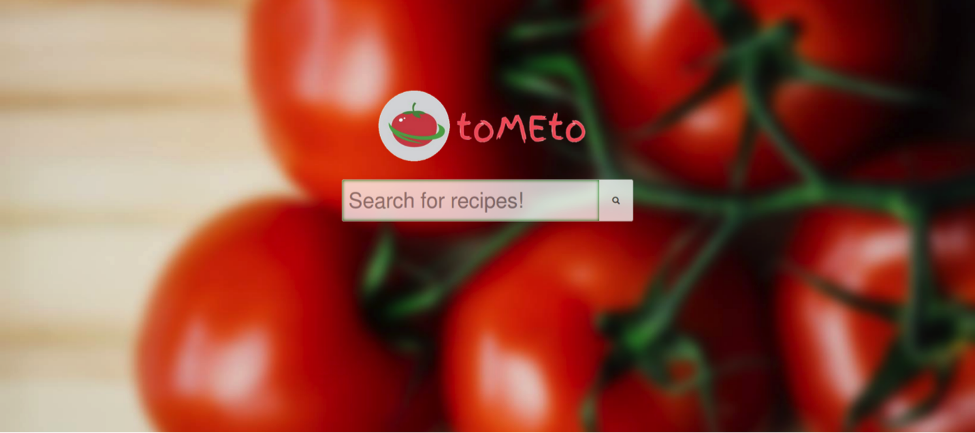
\includegraphics[scale=0.5]{p1.png}

Upon searching for a recipe, a loading bar appears, and once recipe information ins obtained, tiles fade in. These tiles offer an image of the recipe to be prepared, with the recipe title overlaid on top. This can be seen below:

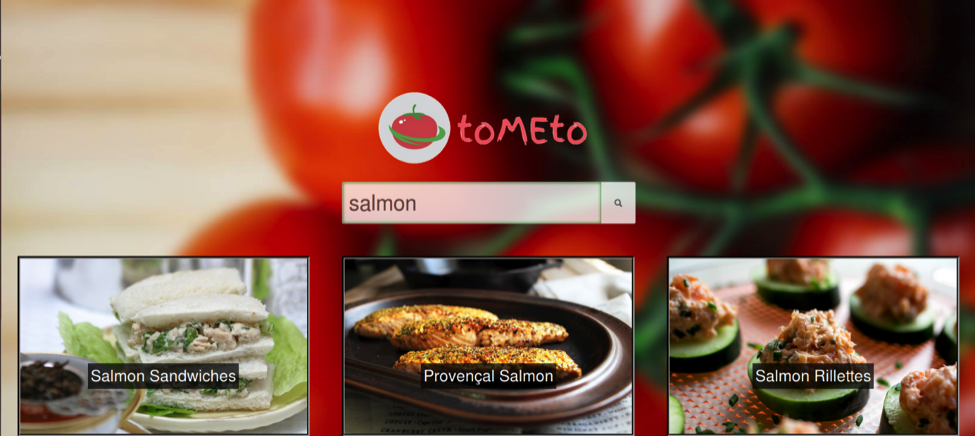
\includegraphics[scale=0.5]{p2.png}

Upon clicking a recipe, a modal popup appears, which lists both the recipe itself as well as toMEto's recommended ingredients, as can be seen in the below image:

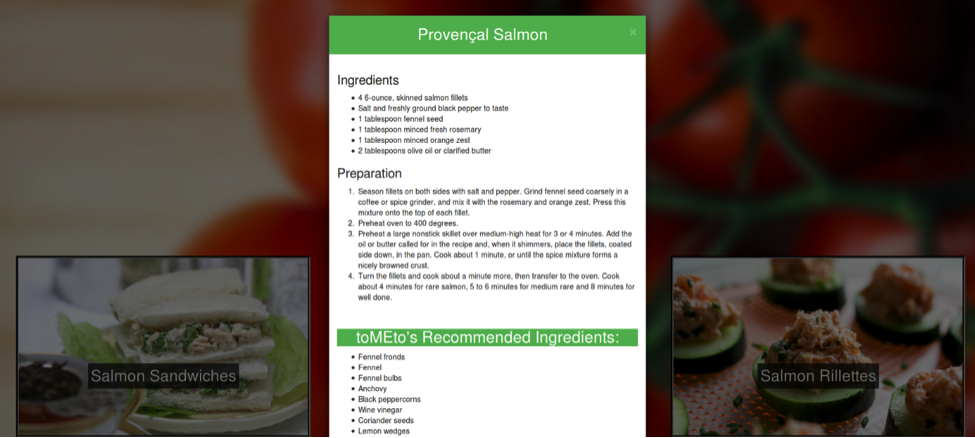
\includegraphics[scale=0.5]{p3.png}

Much of the front-end was designed to be easily updated and maintained, and thus small UI tweaks, such as background images, color schemes, etc. are easily changeable by editing the HTML and/or CSS files. The front-end utilizes mainly three different HTML templates:\begin{itemize}
\item simplesearch.html 
\item simplesearch\_searched.html 
\item no\_results.html
\end{itemize}

simplesearch.html is simply the html for the landing page, before any queries are entered. Then, once a search query is entered, app.py directs this information to the backend, which then generates information which is supplied to the simplesearch\_searched.html template. The user is also redirected to this template, which includes the tiles, modal popup information, etc. Furthermore, if a search is entered into simplesearch\_searched.html, this also refreshes the simplesearch\_searched.html template, utilizing the new information. Finally, no\_results.html is used as a template to be redirected to when the query entered into simplesearch.html or simplesearch\_searched.html does not contain any results. As a note, a user will be redirected to simplesearch.html upon clicking the toMEto logo.

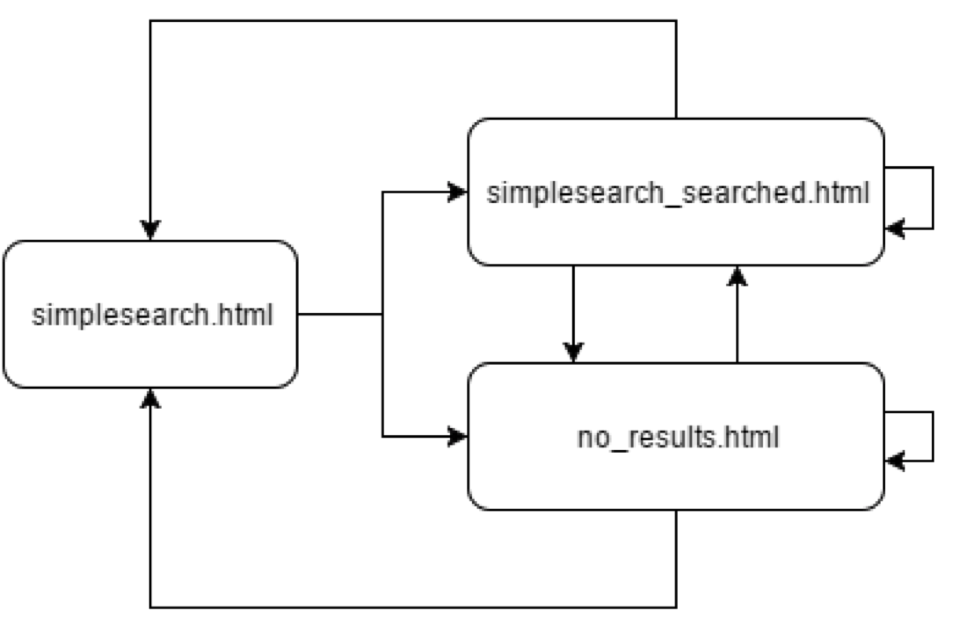
\includegraphics[scale=0.5]{p4.png}


\section{Performance}

Lorem ipsum dolor sit amet, consectetur adipiscing elit, sed do eiusmod tempor incididunt ut labore et dolore magna aliqua. Ut enim ad minim veniam, quis nostrud exercitation ullamco laboris nisi ut aliquip ex ea commodo consequat. Duis aute irure dolor in reprehenderit in voluptate velit esse cillum dolore eu fugiat nulla pariatur. Excepteur sint occaecat cupidatat non proident, sunt in culpa qui officia deserunt mollit anim id est laborum.


\section{Discussion}

Lorem ipsum dolor sit amet, consectetur adipiscing elit, sed do eiusmod tempor incididunt ut labore et dolore magna aliqua. Ut enim ad minim veniam, quis nostrud exercitation ullamco laboris nisi ut aliquip ex ea commodo consequat. Duis aute irure dolor in reprehenderit in voluptate velit esse cillum dolore eu fugiat nulla pariatur. Excepteur sint occaecat cupidatat non proident, sunt in culpa qui officia deserunt mollit anim id est laborum.



\section{Conclusions and Future Work}

Lorem ipsum dolor sit amet, consectetur adipiscing elit, sed do eiusmod tempor incididunt ut labore et dolore magna aliqua. Ut enim ad minim veniam, quis nostrud exercitation ullamco laboris nisi ut aliquip ex ea commodo consequat. Duis aute irure dolor in reprehenderit in voluptate velit esse cillum dolore eu fugiat nulla pariatur. Excepteur sint occaecat cupidatat non proident, sunt in culpa qui officia deserunt mollit anim id est laborum.


%%%%%%%%%%%%%%%%%%%%%%%%%%%%%%%%%%%
%%%% Compiling Instructions %%%%%%%
% pdflatex report.tex
% bibtex report
% pdflatex report.tex
% 
% You have to compile twice to get the references to show up


\bibliographystyle{abbrv}
\bibliography{report}

%\balancecolumns 

\end{document}
